\chapter{Background}
\index{Background@\emph{Background}}\label{background}%
In Section~\ref{back:phylogenetics}, I give a brief introduction to phylogenetics and define basic definitions and concepts that will be used throughout my dissertation.  In Section~\ref{back:hmm}, I describe Hidden Markov Models (HMMs) and their use in alignment estimation. Finally, in Section~\ref{back:metagenomic}, I describe metagenomic analyses and the difficulty in analyzing metagenomic datasets.

\section{Phylogenetics}\label{back:phylogenetics}
\emph{Phylogenetics} is the study of the evolutionary relationship between different organisms.  Often times the product of a phylogenetic study is a \emph{phylogeny}, a hypothesis of the evolutionary history between different species.  One common representation of a phylogeny is through a phylogenetic tree.  Figure~\ref{back:phylo_tree} shows an example of a rooted phylogenetic tree.  
The leaves of the tree represent the organisms of interest.  Throughout my dissertation, I will refer to the leaves of the tree as species, taxa, or sequence, interchangeably.  The relationship between the different species can be inferred from the tree.  For example, species $A$ and $B$ are more closely related than $A$ and $C$ because $A$ and $B$ share a more recent common ancestor (red node) than $A$ and $C$ (blue node).  Each internal node represents a \emph{speciation event}, in which a lineage splits into two new lineages.  The root of the phylogeny represents the most recent common ancestor of all the species.  

The theory of universal common ancestry states that all living organisms have shared evolutionary history, or in other words, all extant species descended from a common ancestor.  Thus, as DNA is passed on from parent to child, DNA and biomolecular sequences that are derived from DNA (RNA and amino acids), are often collected and used to infer phylogenies.  

\textbf{NAM:Add more formal definition, citations; include uses of phylogenies in virology, medicine production, etc..., show unrooted trees, also, discuss models of sequence evolution, indels mutation?}.

\begin{figure}[htpb]
\begin{center}
{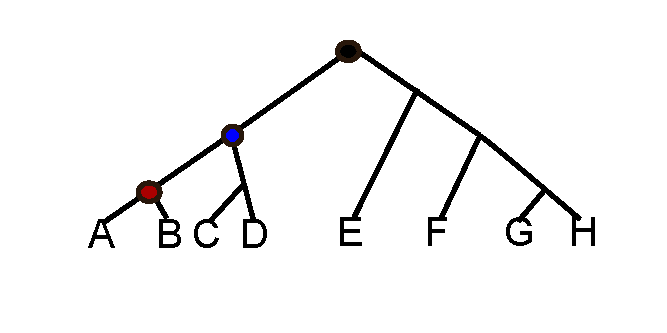
\includegraphics[scale=0.8]{background/phylogeny.pdf}}
\end{center}
\caption[A rooted phylogenetic tree.]{\label{back:phylo_tree} Example of a rooted phylogenetic tree.}
\end{figure}



\subsection{Alignment estimation}\label{back:alignment}

Start with a simplified view of sequence evolution.  There is a DNA sequence at the root.  It evolves down tree through series of substitutions and indels (Fig.~\ref{back:mutations}).  At the end of the process is are sequences that are homologous; they all descended from a common sequence.  A phylogenetic analyses will typically begin by collecting a set of homologous sequences from a common source, such as gene protein sequence.  This is the end result of the sequence evolution process; the history of the changes is lost.  Due to insertion and deletion events, the sequences are all of different length.  Typically a first step in estimating a phylogeny is to first estimate a \emph{Multiple Sequence Alignment} (MSA).  An MSA is a matrix where each row contains a sequence and each column represents shared homology for all biomolecular characters in that column.  

There are many different methods for estimating MSA, including Bayesian techniques (BAli-Phy) that co-estimate alignments and trees, progressive alignment techniques that use a guide tree to pairwise align the sequences (ClustalW, T-COFFEE), iterative methods that use a guide tree, but iterate to obtain better guide trees (Muscle, Mafft, SATe).  

\textbf{NAM:Add more formal definition, citations}.

\subsection{Phylogeny estimation}\label{back:phylogeny}

Once an alignment has been estimated, a phylogeny can be estimated based on various methods such as Maximum Parisomony (TNT and PAUP*), distance-based methods (NJ, UPGMA, FastME), Maximum Likelihood (RAxML, FastTree), or Bayesian methods (Mr. Bayes).  

\textbf{NAM:Add more formal definition, citations}.

\section{Hidden Markov Models}\label{back:hmm}

\textbf{Add text discussing problems of using a single HMM to represent divergent sequences, motivate the HMM families in the next chapter}
\begin{figure}[htbp]
\centering
{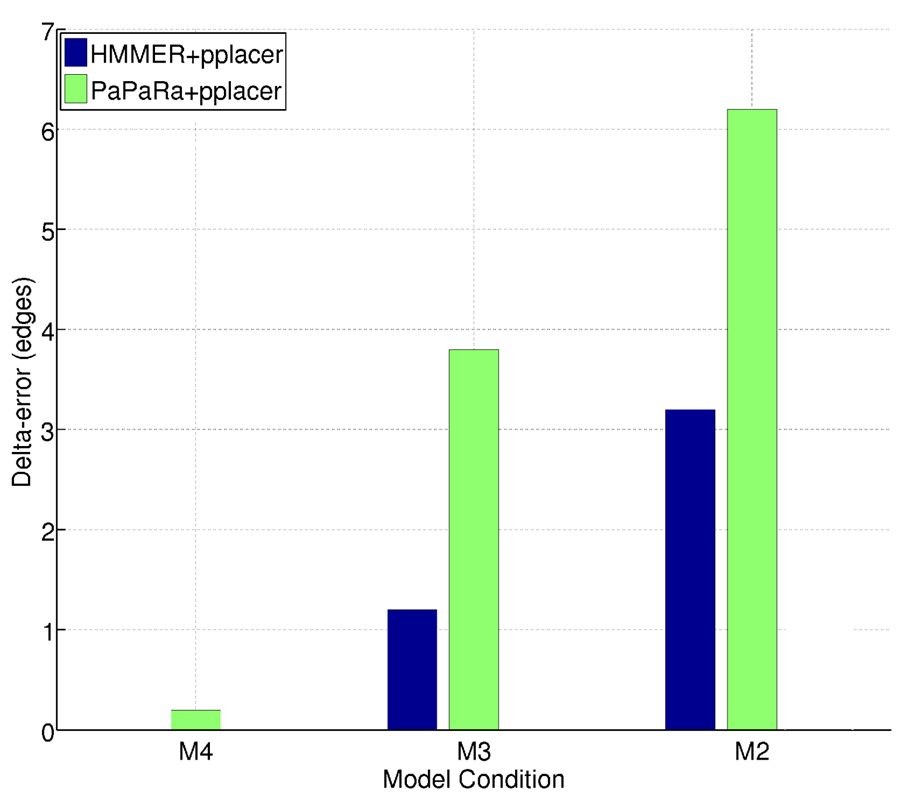
\includegraphics[width=0.80\textwidth]{sepp/hmmer_papara}}
\caption[Comparison of HMMALIGN+pplacer and PaPaRa+pplacer.]{Comparison of HMMALIGN+pplacer and PaPaRa+pplacer under 3 different model conditions, ranked in order of increasing rate of evolution.  Thus, M4 is the slowest evolving dataset, and M2 is the fastest evolving dataset.  The number of sequences in the backbone set is 500 for all model conditions.} 
\label{background:initial}
\end{figure}


\textbf{NAM:Add more formal definition, citations}.
\section{Metagenomic analyses}\label{back:metagenomic}

\textbf{NAM:Add more formal definition, citations}.
\subsection{Taxonomic identification}\label{back:taxonomic_id}

\textbf{NAM:Add more formal definition, citations}.
\subsection{Taxonomic profiling}\label{back:taxonomic_profiling}

\textbf{NAM:Add more formal definition, citations}
